\chapter{Harmonogram realizacji projektu}

\section{Etapy realizacji}

Prace nad projektem zostały podzielone na następujące etapy:

\begin{itemize}
  \item Zatwierdzenie tematu – 17.05.2025,
  \item Analiza i projekt systemu – 18.05–21.05.2025,
  \item Projekt bazy danych i diagram klas – 22.05–24.05.2025,
  \item Implementacja systemu (GUI, DAO, logika) – 25.05–02.06.2025,
  \item Obsługa wyjątków i walidacja – 03.06–05.06.2025,
  \item Testowanie aplikacji – 06.06–08.06.2025,
  \item Tworzenie dokumentacji – 09.06–14.06.2025,
  \item Ostateczne poprawki i złożenie – 15.06.2025.
\end{itemize}

\section{Wizualizacja harmonogramu}

Poniżej przedstawiono diagram Gantta obrazujący kolejne etapy realizacji projektu:

\begin{figure}[H]
\centering
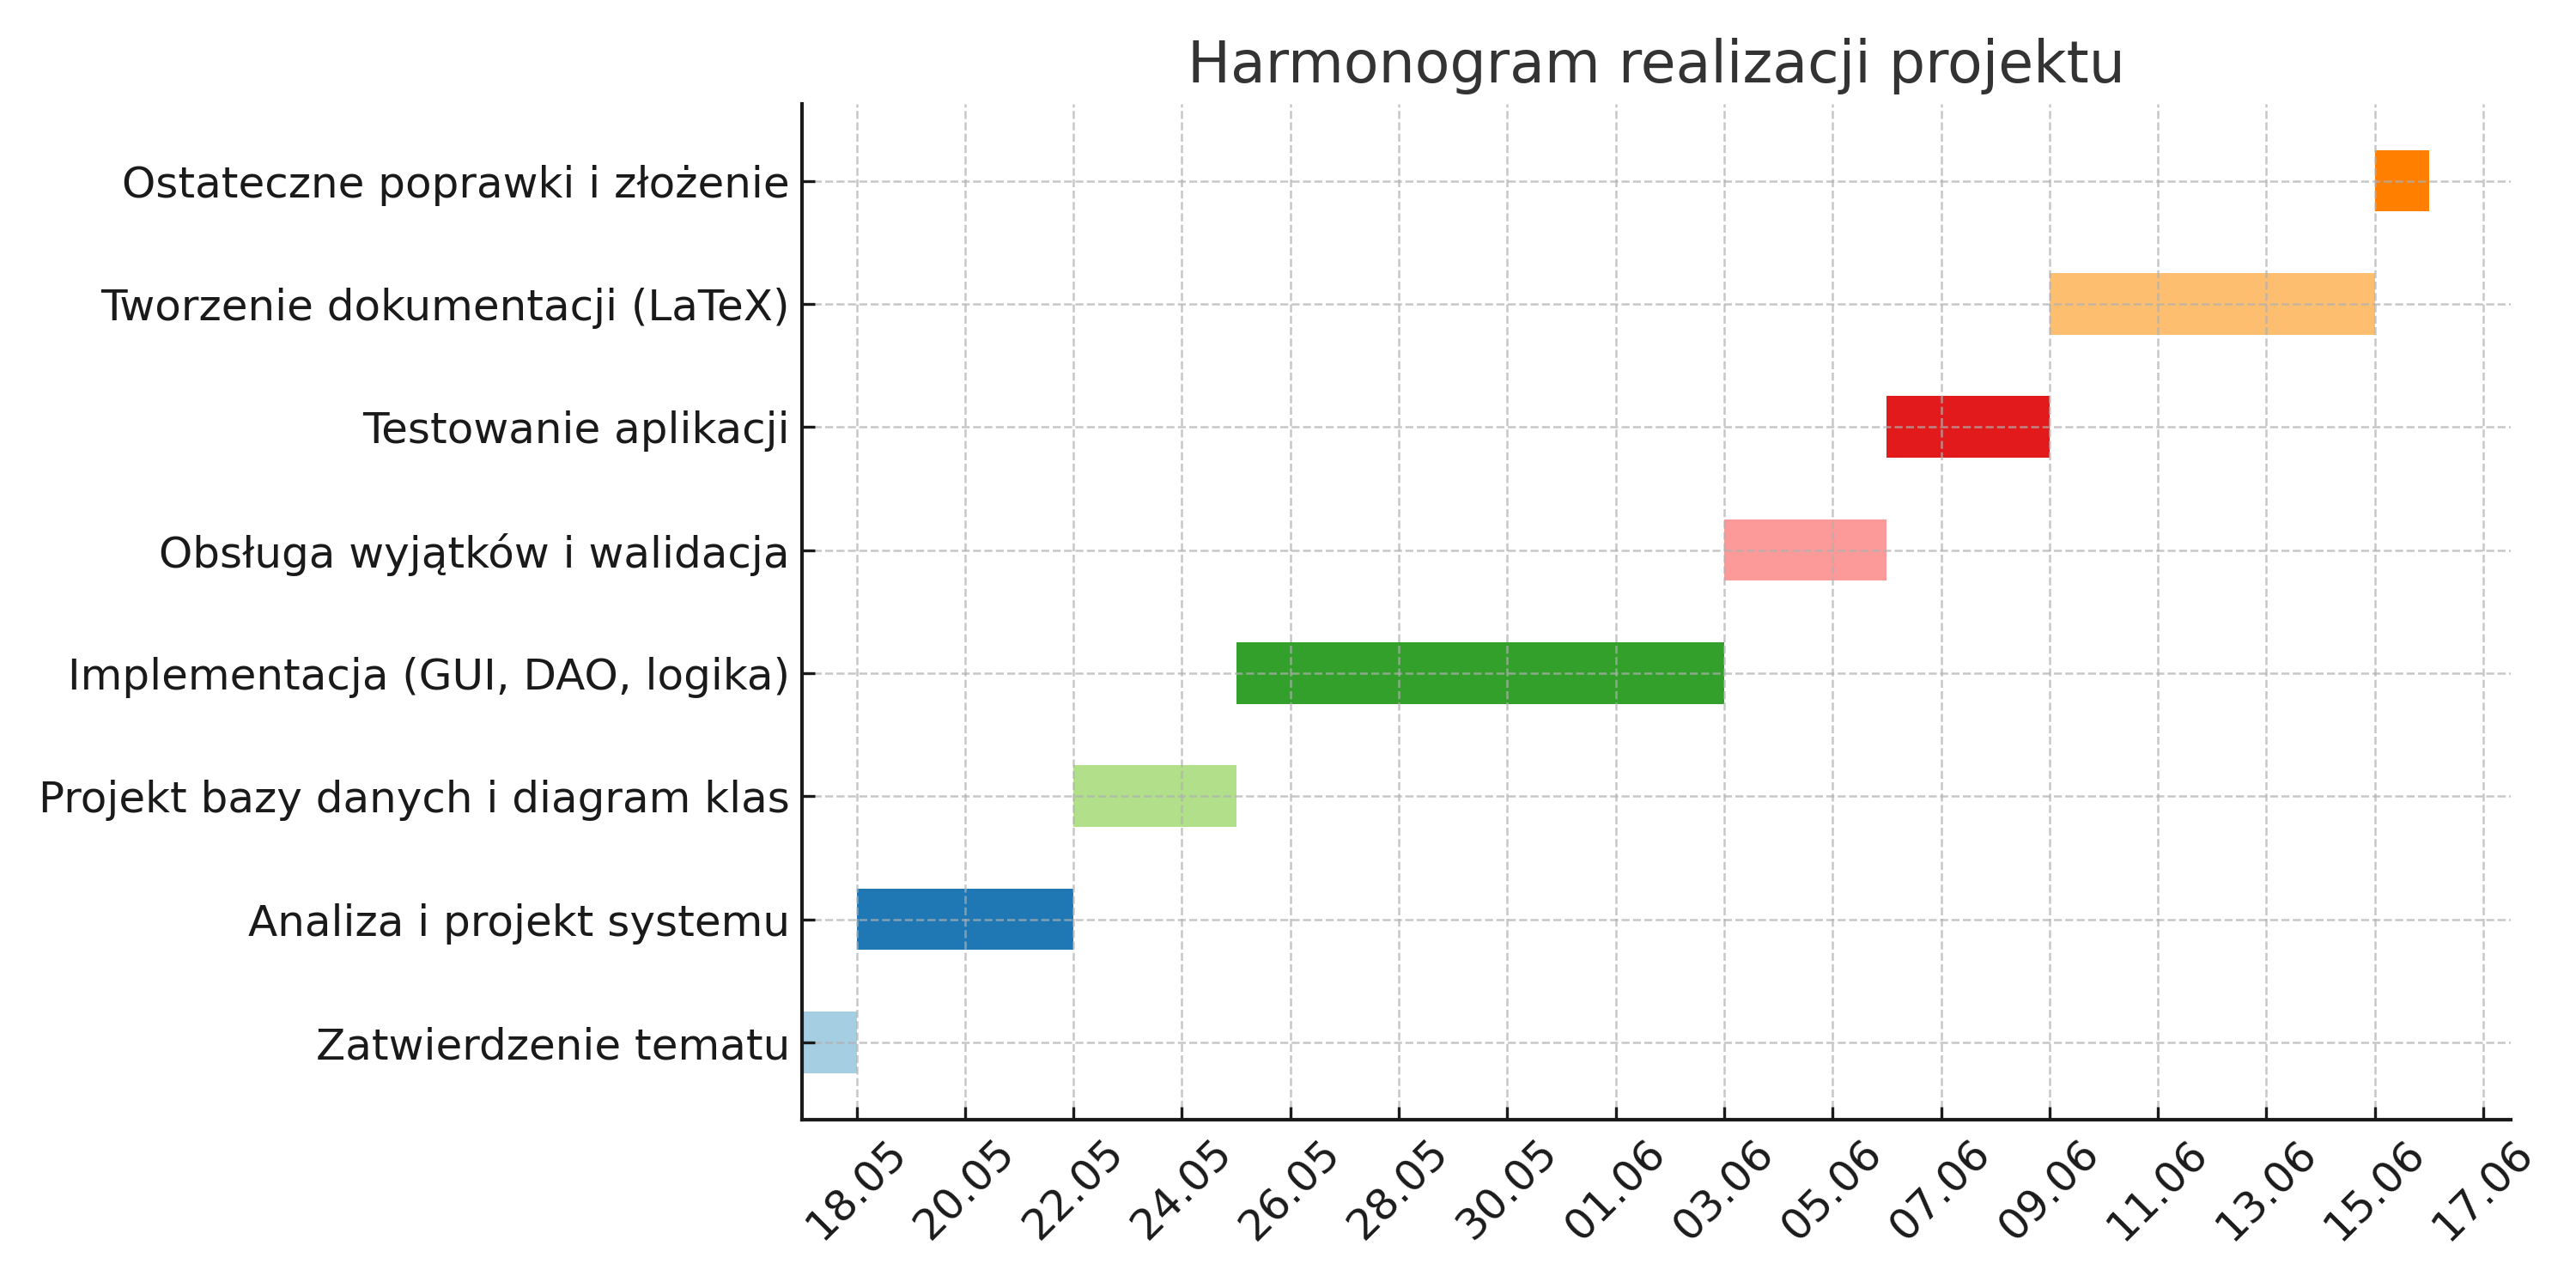
\includegraphics[width=0.95\textwidth]{figures/harmonogram_gantta.png}
\caption{Diagram Gantta – harmonogram realizacji projektu}
\end{figure}
